\section{Problem 1}
\subsection{a}
IN RMS, the static priorities are assigned according to the cycle duration of the job, so a shorter cycle duration results in a higher job priority, so it sets Task1 higher priority than Task2.
\begin{figure}[H]
 \centering
 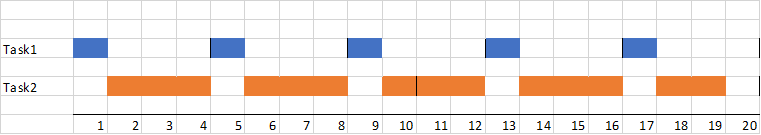
\includegraphics[width=0.9\textwidth]{images/rate-monotonicschedule.png}
 \caption{Rate-monotonic schedule}
 \label{a}
\end{figure}

\subsection{b}

\begin{figure}[H]
 \centering
 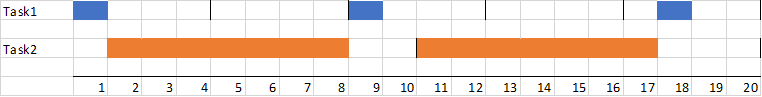
\includegraphics[width=0.9\textwidth]{images/mutex.png}
 \caption{With mutex}
 \label{b}
\end{figure}

From the picture \ref{b} we can see if the mutex is introduced, the deadline cannot always meet, which means is not feasible.

\subsection{c}

Using the Liu-Layland-Criteria(lecture 12, page 20):
\begin{equation}
    \begin{aligned}
        &U \equiv \sum_i^N\frac{C_i}{T_i}\leq N(2^{1/N}-1)\\
        &\Rightarrow\frac{1}{4} + \frac{e_2}{10}\leq 2(2^{1/2} -1)\\
        &\Rightarrow e_2 \leq 5.78
    \end{aligned}
\end{equation}

This means if the execution time of Task 2 is less or equal to 5 units, it can be feasible.

The schedule is shown in figure \ref{c}:

\begin{figure}[H]
 \centering
 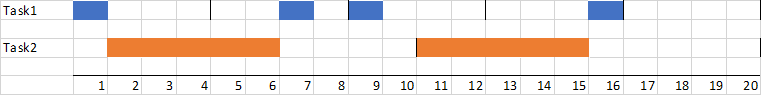
\includegraphics[width=0.9\textwidth]{images/anytime.png}
 \caption{Schedule with anytime algorithm}
 \label{c}
\end{figure}

\subsection{d}

In EDF, whenever a scheduling event occurs (task finishes, new task released, etc.) the queue will be searched for the process closest to its deadline. This process is the next to be scheduled for execution.

The schedule for EDF is shown below:

\begin{figure}[H]
 \centering
 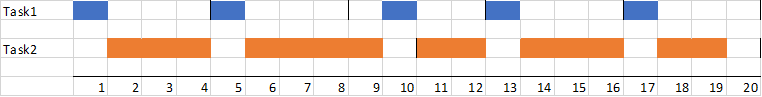
\includegraphics[width=0.9\textwidth]{images/EDF.png}
 \caption{EDF schedule}
 \label{EDF}
\end{figure}

\subsection{e}
EDF test criterion is(from lecture 12 page 32):
\begin{equation}
    \begin{aligned}
        &\sum_{i=1}^N\frac{C_i}{T_i}\le1\\
        &\Rightarrow \frac{1}{4}+\frac{e_2}{10} +\frac{2}{5} \leq 1\\
        &\Rightarrow e_2 \leq 3.5
    \end{aligned}
\end{equation}

This says $ e_{2-max} = 3 $ units.

And the schedule figure is shown below:

\begin{figure}[H]
 \centering
 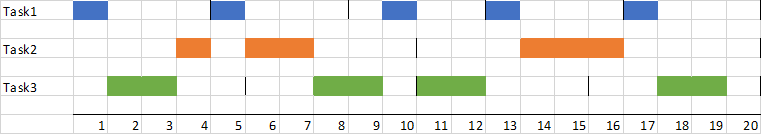
\includegraphics[width=0.9\textwidth]{images/EDFe.png}
 \caption{EDf for 3 tasks}
 \label{label}
\end{figure}
